
\exo

\emph{Donner les réponses sous forme d'une fraction, sous forme décimale, et sous forme d'un pourcentage.}
\begin{enumerate}
\item Parmi les $500$ étudiants inscrits dans un conservatoire, $320$ pratiquent le piano.

Quelle est la proportion d'étudiants pratiquant le piano parmi les étudiants de ce conservatoire ?
\item Un maraîcher a rempli sa camionnette de $70$ cageots, dont $49$ sont des cageots de fruits.

Quelle est la proportion de cageots de fruits parmi l'ensemble des cageots ?
\item En juin 2017, l'Assemblée nationale comportait $224$ femmes députées sur les $577$ élus.

Quelle était la proportion de femmes députées à l'Assemblée nationale ?
\end{enumerate}

\exo

\begin{enumerate}
\item Un paquet de pâtes de $500$ grammes contient \SI{60}{\percent} de pâtes colorées.

Quelle est la masse de pâtes colorées dans ce paquet ?
\item Le 12 juillet 2021 en France, \np{26863140} personnes avaient reçu un schéma vaccinal complet contre le Covid-19. Elles représentaient alors \SI{41,7}{\percent} de la population.

Quelle était la population en France à cette date ?
\end{enumerate}

\exo

La classe de 2\up{nde} 9 compte $24$ élèves. Deux tiers de ces élèves sont demi-pensionnaires, quinze sont des filles, et cette classe représente \SI{2}{\percent} de l'effectif du lycée.

Imaginer trois questions, et donner leurs réponses.

\exo

\begin{enumerate}
\item La carte d'un restaurant est composée pour moitié de plats. Parmi eux, \SI{20}{\percent} sont végétariens.

Déterminer la proportion de plats végétariens dans la carte de ce restaurant.
\item Un concessionnaire a remarqué que \SI{80}{\percent} de ses ventes sont des utilitaires. Parmi ceux-ci, \SI{35}{\percent} sont de couleur blanche.

Déterminer la proportion d'utilitaires blancs parmi les ventes de ce concessionnaire.
\item  Dans une classe, \SI{45}{\percent} des élèves sont des garçons. Parmi eux, \SI{20}{\percent} portent des lunettes.

Déterminer la proportion de garçons portant des lunettes dans l'ensemble de la classe.
\end{enumerate}

\exo

Lors d'une enquête réalisée auprès de $800$ garçons et $1200$ filles, on a obtenu les résultats suivants :
\begin{itemize}
\item parmi les garçons :
\begin{itemize}
\item \SI{5}{\percent} passent leurs vacances d'été chez eux ;
\item \SI{20}{\percent} partent à l'étranger ;
\item tous les autres partent dans une région française différente de la leur.
\end{itemize}
\item parmi les filles :
\begin{itemize}
\item \SI{7}{\percent} passent leurs vacances d'été chez elles ;
\item \SI{15}{\percent} partent à l'étranger ;
\item toutes les autres partent dans une région française différente de la leur.
\end{itemize}
\end{itemize}
\begin{enumerate}
\item Compléter le tableau suivant, en indiquant des effectifs :
\begin{center}
\setlength{\tabcolsep}{0.1cm}
\renewcommand{\arraystretch}{1.2}
\begin{tabular}{
|>{\raggedright\arraybackslash}m{3cm}
*{3}{|>{\centering\arraybackslash}m{3cm}}|}
\hline 
& \textbf{Garçons} & \textbf{Filles} & \textbf{Total} \\ 
\hline
\textbf{Chez eux} &  &  &  \\ 
\hline 
\textbf{À l'étranger} &  &  &  \\ 
\hline 
\textbf{Autre région} &  &  &  \\ 
\hline 
\textbf{Total} &  &  &  \\ 
\hline 
\end{tabular} 
\end{center}
\item Quelle proportion de garçons partent dans une région autre que la leur, dans la population des garçons ?
\item Quelle proportion de filles partent à l'étranger, dans la population totale ?
\end{enumerate}

\exo

\begin{enumerate}
\item Lorsqu'Alice prend une boisson à la machine automatique, il s'agit d'un café la moitié du temps. Lorsqu'elle prend un café, elle y ajoute du sucre une fois sur trois.

Déterminer la proportion de cafés sucrés parmi les boissons prises par Alice.
\item Bob utilise un site de vidéos en streaming. Il a remarqué que parmi toutes les vidéos qu'il visionne, \SI{35}{\percent} sont des séries, et que \SI{7}{\percent} sont des séries françaises.

Déterminer la proportion de séries françaises parmi les séries regardées par Bob.
\item  Une étude de l'INSEE a relevé qu'en 2016, \SI{19,3}{\percent} des salariés travaillaient à temps partiel. Selon la même étude, la proportion de femmes salariées à temps partiel parmi l'ensemble des salariés est alors de \SI{15,4}{\percent}.

Déterminer la proportion de femmes parmi les salariés à temps partiel en 2016.
\end{enumerate}

\exo

Le nombre d'abonnés d'un journal passe de \np{6300} à \np{5400}.
\begin{enumerate}
\item Déterminer la variation absolue du nombre d'abonnés.
\item Déterminer le taux de cette évolution en pourcentage.
\end{enumerate}

\exo

En 1927, Charles \textsc{Lindbergh} réalisa le premier vol New York - Paris sans escale, en 33 heures et 30 minutes. Cinquante ans plus tard, le \textit{Concorde} effectuait le même trajet en 3 heures et 27 minutes.

Déterminer le taux d'évolution de ce temps de vol, en pourcentage.

\exo

Voici l'évolution de la moyenne générale d'un élève au cours de l'année :
\begin{center}
\setlength{\tabcolsep}{0.1cm}
\renewcommand{\arraystretch}{1.2}
\begin{tabular}{
*{3}{>{\centering\arraybackslash}m{2.5cm}}}
\hline 
$1$\ier{} trimestre & $2$\ieme{} trimestre & $3$\ieme{} trimestre \\ 
\hline
$12,3$ & $13,5$ & $10,6$ \\ 
\hline 
\end{tabular} 
\end{center}
\begin{enumerate}
\item Déterminer la variation absolue de cette moyenne entre le premier et le deuxième trimestre.
\item Déterminer sa variation relative en pourcentage, entre le premier et le deuxième trimestre, puis entre le deuxième et le troisième trimestre.
\end{enumerate}

\exo

Déterminer les coefficients multiplicateurs associés aux évolutions suivantes :

\vspace{-12pt}
\setlength{\columnsep}{1cm}
\setlength{\columnseprule}{0pt}
\begin{multicols}{2}
\begin{enumerate}
\item une augmentation de \SI{10}{\percent}.
\item une diminution de \SI{10}{\percent}.
\item une augmentation de \SI{45}{\percent}.
\item une augmentation de \SI{2,3}{\percent}.
\item une diminution de \SI{0,3}{\percent}.
\item une augmentation de \SI{100}{\percent}.
\item une diminution de \SI{5}{\percent}.
\item une augmentation de \SI{1,03}{\percent}.
\item une augmentation de \SI{300}{\percent}.
\item une diminution de \SI{95}{\percent}.
\end{enumerate}
\end{multicols}
\vspace{-12pt}

\exo

Déterminer les taux d'évolution en pourcentage associés aux coefficients multiplicateurs suivants :

\vspace{-12pt}
\setlength{\columnsep}{1cm}
\setlength{\columnseprule}{0pt}
\begin{multicols}{4}
\begin{enumerate}
\item $k=1,2$.
\item $k=0,89$.
\item $k=1,03$.
\item $k=2$.
\item $k=0,3$.
\item $k=1,0087$.
\item $k=3,32$.
\item $k=0,876$.
\end{enumerate}
\end{multicols}
\vspace{-12pt}

\exo

\begin{enumerate}
\item Lorsqu'il est entré en 2\up{nde}, Léo mesurait \SI{1,60}{\m}. Au cours de l'année, sa taille a augmenté de \SI{5}{\percent}.

Quelle était la taille de Léo à la fin de l'année ?
\item Pendant les vacances scolaires, Léna jouait chaque jour sur sa console, pendant 1 heure et 40 minutes. À la rentrée, ses parents lui ont demandé de réduire son temps de jeu de \SI{80}{\percent}.

Combien de temps joue-t-elle chaque jour, maintenant ?
\item Une veste est vendue $120$ euros.
\begin{enumerate}
\item Lors d'une promotion, son prix diminue de \SI{30}{\percent}. Quel est son nouveau prix ?
\item À l'occasion d'une deuxième démarque, son prix diminue encore à $58,80$ euros.

Quel est le taux de la deuxième réduction, en pourcentage ?
\end{enumerate}
\end{enumerate}

\exo

Le tableau ci-dessous donne le tarif du ticket restaurant (en euros), de 2016 à 2019 :
\begin{center}
\setlength{\tabcolsep}{0.1cm}
\renewcommand{\arraystretch}{1.2}
\begin{tabular}{
*{5}{|>{\centering\arraybackslash}m{3cm}}|}
\hline 
Année & 2016 & 2017 & 2018 & 2019 \\ 
\hline
Tarif 	& $8,60$ & $8,66$ & $8,73$ & $8,73$ \\
\hline 
\end{tabular} 
\end{center}
Calculer le taux d'évolution du tarif du ticket-restaurant (en \si{\percent}, arrondi au dixième de point) :

\vspace{-12pt}
\setlength{\columnsep}{1cm}
\setlength{\columnseprule}{0pt}
\begin{multicols}{3}
\begin{itemize}
\item de 2017 à 2018 ;
\item de 2018 à 2019 ;
\item de 2016 à 2019.
\end{itemize}
\end{multicols}



\exo

Compléter le tableau suivant :
\begin{center}
\setlength{\tabcolsep}{0.1cm}
\renewcommand{\arraystretch}{1.2}
\begin{tabular}{
*{5}{|>{\centering\arraybackslash}m{3cm}}|}
\hline 
& Stock initial (en~kg) & Stock final (en~kg) & Évolution (\si{\percent}) & Coefficient multiplicateur \\ 
\hline
Tomates 	& $45,2$&		&		& $1,12$ \\ 
\hline 
Aubergines 	& $80$ 	& $97$	&		& 				\\ 
\hline 
Courgettes 	&      	& $12$	&		& $0,6$ \\ 
\hline 
Oignons 	& $16$	& 		& \SI{-8}{\percent}	&	\\ 
\hline 
Carottes 	&		& $115$	& \SI{-20}{\percent}&	\\ 
\hline 
\end{tabular} 
\end{center}

\exo

Voici une feuille de calcul créée sur un tableur.

Quelle formule faut-il saisir dans la cellule \textsf{B3}, et recopier vers la droite, pour obtenir la dernière ligne de ce tableau ?
\begin{center}
\definecolor{grisfonce}{RGB}{180,180,180}
\definecolor{grisclair}{RGB}{230,230,230}
\begin{sffamily}
\setlength{\tabcolsep}{0.7mm}
\renewcommand{\arraystretch}{1.2}
\begin{tabular}{>{\columncolor{grisclair}\centering\arraybackslash}m{5mm}
|>{\centering\arraybackslash}m{30mm}
*{6}{|>{\centering\arraybackslash}m{15mm}}|}
\rowcolor{grisclair}
\multicolumn{1}{r|}{\raisebox{-1mm}{
\psset{unit=0.35cm}\begin{pspicture*}(0,0)(1,1)\pspolygon[linewidth=0pt, linecolor=grisfonce, fillcolor=grisfonce, fillstyle=solid](0,0)(1,0)(1,1)\end{pspicture*}}} & A & B & C & D & E & F & G \\ 
\hline
1 & Valeur initiale & 140 & 140 & 140 & 140 & 140 & 140 \\ 
\hline 
2 & Taux (en \si{\percent}) & -3 & -2 & -1 & 1 & 2 & 3 \\ 
\hline 
3 & Valeur finale & 135,8 & 137,2 & 138,6 & 141,4 & 142,8 & 144,2 \\ 
\hline 
\end{tabular} 
\end{sffamily}
\end{center}

\exo

Le prix d'un article a augmenté de \SI{5}{\percent} puis de \SI{10}{\percent}.
\begin{enumerate}
\item Déterminer les coefficients multiplicateurs associés à ces deux augmentations.
\item En déduire le coefficient multiplicateur global, puis le taux d'évolution global de ce prix.
\end{enumerate}

\exo

On étudie l'évolution de la population d'une ville pendant plusieurs années :
\begin{center}
\setlength{\tabcolsep}{0.1cm}
\renewcommand{\arraystretch}{1.2}
\begin{tabular}{
*{4}{>{\centering\arraybackslash}m{3cm}}}
\hline 
\textbf{Période} & 2015-2016 & 2016-2017 & 2017-2018 \\ 
\hline
\textbf{Évolution} & \SI[retain-explicit-plus]{+2}{\percent} & \SI[retain-explicit-plus]{-6}{\percent} & \SI[retain-explicit-plus]{+8}{\percent} \\ 
\hline 
\end{tabular}
\end{center}
\begin{enumerate}
\item Justifier que la population a globalement diminué de \SI[retain-explicit-plus]{4,12}{\percent} sur la période 2015-2017.
\item Justifier que la population a globalement augmenté de \SI[retain-explicit-plus]{1,52}{\percent} sur la période 2016-2018.
\item Déterminer le taux d'évolution global sur la période 2015-2018.
\end{enumerate}

\exo

Le coût de fabrication d'un objet a augmenté de \SI{24}{\percent}, puis il a diminué de \SI{17}{\percent}.

L'évolution globale est-elle une augmentation ou une diminution ? Quel est son taux ?

\exo

Les affirmations suivantes sont-elles vraies ou fausses ? Justifier la réponse.
\begin{enumerate}
\item Une augmentation de \SI[retain-explicit-plus]{10}{\percent} suivie d'une augmentation de \SI[retain-explicit-plus]{20}{\percent} correspondent à une augmentation de globale de \SI[retain-explicit-plus]{50}{\percent}.
\item Deux diminutions successives de \SI[retain-explicit-plus]{30}{\percent} correspondent à une diminution globale de \SI[retain-explicit-plus]{51}{\percent}.
\end{enumerate}

\exo

En Syldavie, l'inflation a été de \SI[retain-explicit-plus]{4}{\percent} en 2017, puis de \SI[retain-explicit-plus]{3}{\percent} en 2018. En Bordurie, elle a été de \SI[retain-explicit-plus]{5}{\percent} en 2017, puis de \SI[retain-explicit-plus]{2}{\percent} en 2018.

Dans quel pays les prix ont-il le plus augmenté sur l'ensemble de ces deux années ?

\exo

\vspace{-12pt}
\setlength{\columnsep}{1cm}
\setlength{\columnseprule}{0pt}
\begin{multicols}{2}
On considère la fonction Python ci-contre.
\begin{enumerate}
\item Quelle sera la valeur renvoyée par l'appel :
\begin{pythonconsole}
>>> mystere(20, -40)
\end{pythonconsole}
\item Si \pythoninline{t1/100} et \pythoninline{t2/100} représentent des taux d'évolution, que représente la variable \pythoninline{k} ?
\end{enumerate}
\columnbreak
\begin{pythoncodenumligne}
def mystere(t1, t2):
    k = (1 + t1/100) * (1 + t2/100)
    return k
\end{pythoncodenumligne}
\end{multicols}
\vspace{-12pt}

\exo

Compléter chaque schéma :
\begin{center}
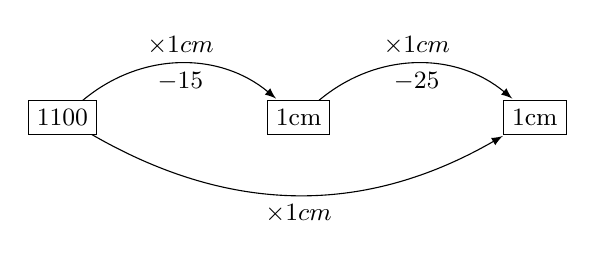
\begin{tikzpicture}[->,>=latex,shorten >=1pt]
\begin{small}
\node[draw,rectangle] (1) at (0,0) {$1100$};
\node[draw,rectangle] (2) at (3,0) {\vphantom{$1$}\dotrule{1cm}};
\node[draw,rectangle] (3) at (6,0) {\vphantom{$1$}\dotrule{1cm}};
\draw
    (1) edge [out=40,in=140] node[below] {$-\SI{15}{\percent}$} node[above] {$\times\vphantom{1}\dotrule{1cm}$} (2)
    (1) edge [out=330,in=210] node[below] {$\times\vphantom{1}\dotrule{1cm}$} (3)
    (2) edge [out=40,in=140] node[below] {$-\SI{25}{\percent}$} node[above] {$\times\vphantom{1}\dotrule{1cm}$} (3) ;
\end{small}
\end{tikzpicture}
\qquad
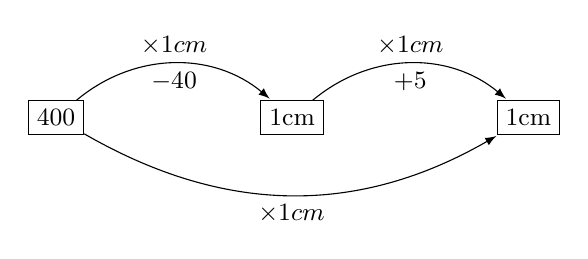
\begin{tikzpicture}[->,>=latex,shorten >=1pt]
\begin{small}
\node[draw,rectangle] (1) at (0,0) {$400$};
\node[draw,rectangle] (2) at (3,0) {\vphantom{$1$}\dotrule{1cm}};
\node[draw,rectangle] (3) at (6,0) {\vphantom{$1$}\dotrule{1cm}};
\draw
    (1) edge [out=40,in=140] node[below] {$-\SI{40}{\percent}$} node[above] {$\times\vphantom{1}\dotrule{1cm}$} (2)
    (1) edge [out=330,in=210] node[below] {$\times\vphantom{1}\dotrule{1cm}$} (3)
    (2) edge [out=40,in=140] node[below] {$+\SI{5}{\percent}$} node[above] {$\times\vphantom{1}\dotrule{1cm}$} (3) ;
\end{small}
\end{tikzpicture}
\end{center}
\vspace{-6pt}

\exo

En 2020, un village comptait $700$ habitants. Suite à la fermeture d'une usine, \SI{8}{\percent} des habitants du village sont partis. Heureusement, avec l'arrivée du TGV en 2022, le maire prévoit une augmentation de \SI{25}{\percent} de la population.

Calculer le coefficient multiplicateur global, et en déduire le nombre prévisible d'habitants en 2022.

\exo

Une caméra \og sport \fg{} au prix de $320$ \euro{} est soldée de \SI{12}{\percent}. Une carte de fidélité permet d'avoir \SI{10}{\percent} de remise supplémentaire.
\begin{enumerate}
\item Calculer le coefficient multiplicateur global.
\item En déduire le prix de cette caméra après ces remises.
\end{enumerate}

\exo

En 2022, le taux d'intérêt du livret A est \SI{1}{\percent} par an.
\begin{enumerate}
\item Alice place \np{1200} \euro{} sur un livret A. Quelle somme aura-t-elle sur ce compte en 2023 ?
\item En supposant que ce taux reste constant et qu'Alice n'ajoute pas d'argent sur ce livret, quelle somme, arrondie au centime, aura-t-elle sur ce compte en 2025 ? En 2029 ?
\end{enumerate}

\exo

Un prix subit une diminution de \SI{25}{\percent} puis une évolution de $t$ \si{\percent}. Globalement, il augmente de \SI{3,5}{\percent}.

Déterminer le taux, en pourcentage, de la seconde évolution.

\exo

Entre son édition \og classique \fg{}  et son édition \og poche \fg{}, l'épaisseur d'un livre a diminué de \SI{36}{\percent}.
\begin{enumerate}
\item Déterminer le taux d'augmentation de l'épaisseur entre l'édition \og poche \fg{} et l'édition \og classique \fg{}.
\item L'édition \og luxe \fg{} a une épaisseur de \SI{4,6}{\cm}. Cette édition est \SI{15}{\percent} plus épaisse que l'édition \og classique \fg{}. Quelle est l'épaisseur de l'édition \og classique \fg{} ?
\end{enumerate}

\exo

Compléter chaque schéma :
\begin{center}
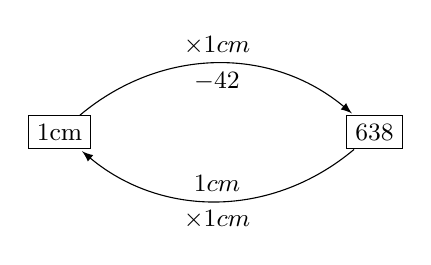
\begin{tikzpicture}[->,>=latex,shorten >=1pt]
\begin{small}
\node[draw,rectangle] (1) at (0,0) {\vphantom{$1$}\dotrule{1cm}};
\node[draw,rectangle] (2) at (4,0) {$638$};
\draw
    (1) edge [out=40,in=140] node[below] {$-\SI{42}{\percent}$} node[above] {$\times\vphantom{1}\dotrule{1cm}$} (2)
    (2) edge [out=220,in=320] node[below] {$\times\vphantom{1}\dotrule{1cm}$} node[above] {$\vphantom{1}\dotrule{1cm}$\si{\percent}} (1) ;
\end{small}
\end{tikzpicture}
\qquad
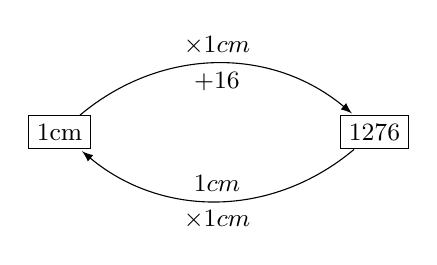
\begin{tikzpicture}[->,>=latex,shorten >=1pt]
\begin{small}
\node[draw,rectangle] (1) at (0,0) {\vphantom{$1$}\dotrule{1cm}};
\node[draw,rectangle] (2) at (4,0) {$1276$};
\draw
    (1) edge [out=40,in=140] node[below] {$+\SI{16}{\percent}$} node[above] {$\times\vphantom{1}\dotrule{1cm}$} (2)
    (2) edge [out=220,in=320] node[below] {$\times\vphantom{1}\dotrule{1cm}$} node[above] {$\vphantom{1}\dotrule{1cm}$\si{\percent}} (1) ;
\end{small}
\end{tikzpicture}
\end{center}
\vspace{-6pt}

\exo

Un magasin d'électroménager propose de rembourser la TVA à ses clients.

Si le taux de TVA est \SI{20}{\percent}, quel est le taux de la remise offerte aux clients ?

\exo

Le taux de TVA en France est de \SI[retain-explicit-plus]{20}{\percent}, et le prix TTC d'un réfrigérateur est de 450 euros.

Quel est le prix hors taxes de ce réfrigérateur ?

\exo

Les affirmations suivantes sont-elles vraies ou fausses ? Justifier la réponse.
\begin{enumerate}
\item L'évolution réciproque d'une diminution de \SI{37,5}{\percent} est une augmentation de \SI{60}{\percent}.
\item Si, après une réduction de \SI{30}{\percent}, un article vaut $154$ \euro{}, il suffit de diviser $154$ par $0,3$ pour retrouver le prix avant la réduction.
\end{enumerate}

\exo

Lors des soldes, le prix d'un pantalon a bénéficié d'une première remise de \SI[retain-explicit-plus]{50}{\percent}. Une remise supplémentaire de \SI[retain-explicit-plus]{20}{\percent} est accordée aux clients fidèles.
\begin{enumerate}
\item Déterminer le taux global de la réduction accordée aux clients fidèles.
\item Le prix du pantalon après la première réduction est $62,60$ euros.

Déterminer son prix initial, et le prix payé par les clients fidèles.
\end{enumerate}

\exo

Un site de vente par Internet réalise une étude statistique des connexions au site afin d'anticiper la puissance de ses serveurs dans les années à venir.

Le tableau ci-dessous récapitule le nombre moyen de connexions par jour, calculé sur une année, pour les années 2015 à 2018.
\begin{center}
\setlength{\tabcolsep}{0.1cm}
\renewcommand{\arraystretch}{1.2}
\begin{tabular}{
>{\raggedright\arraybackslash}m{3cm}
*{5}{>{\centering\arraybackslash}m{1.5cm}}}
\hline 
\textbf{Année} & 2015 & 2016 & 2017 & 2018 \\ 
\hline
\textbf{Connexions} & \np{2678} & \np{2879} & \np{3095} & \np{3327} \\ 
\hline 
\end{tabular} 
\end{center}
\begin{enumerate}
\item Calculer le taux d'évolution de la fréquentation entre 2015 et 2016. Donner le résultat pourcentage arrondi à \SI[retain-explicit-plus]{0,1}{\percent} près.
\item Calculer de même les taux d'évolution de cette fréquentation entre 2016 et 2017, puis entre 2017 et 2018.

Que peut-on constater ?
\item Calculer de deux manières différentes le taux d'évolution, arrondi à \SI[retain-explicit-plus]{0,1}{\percent} près, de la fréquentation entre 2015 et 2018.
\item On suppose que la fréquentation de ce site a aussi augmenté de \SI[retain-explicit-plus]{7,5}{\percent} entre 2014 et 2015. Déterminer à la fréquentation de ce site, arrondie à l'unité, en 2014.
\end{enumerate}

\exo

Une banque propose un placement à intérêts composés : chaque année, les intérêts acquis sont intégrés au capital et fournissent eux-mêmes des intérêts.

On place \np{15000} \euro{}, et deux ans plus tard, le montant disponible est \np{16224} \euro{}.

Quel est le taux annuel de ce placement ?

\exo

Un prix subit deux baisses consécutives de $t$ \si{\percent}, qui correspondent à une baisse globale de \SI{64}{\percent}.

Quelle est la valeur de $t$ ?

\exo

Un refuge de la SPA ne recueille que des chiens et des chats.

En un an, le nombre de chiens a augmenté de \SI{60}{\percent}, alors que le nombre de chats a diminué de \SI{60}{\percent} ; il se trouve qu'ainsi, les proportions de chiens et de chats ont été échangées.

De quel pourcentage a diminué le nombre total d'animaux du refuge ?
